\chapter{Valuation de Empreendimentos Tecnológicos e Projetos de Impacto}
\label{cap:14}

\noindent\tagAV{AV2 (20\%)}\ \tagQuant
\vspace{6pt}

\begin{capObjetivos}
Ao concluir este capítulo, você será capaz de:
\begin{enumerate}[leftmargin=1.4em, itemsep=2pt]
  \item Distinguir \textbf{preço} (negociação de mercado) de \textbf{valor intrínseco} (capacidade de geração de caixa futuro ajustada ao risco) no processo de \textit{Valuation}.
  \item Calcular o Custo Médio Ponderado de Capital (\textbf{WACC}), o \textbf{Valor Terminal} pela perpetuidade de Gordon, o \textbf{Enterprise Value (EV)} e a passagem para o \textbf{Equity Value} no modelo de Fluxo de Caixa Descontado (Damodaran, 2010).
  \item Reconhecer os desafios de avaliar empresas jovens e sem histórico contábil (\textit{The Dark Side of Valuation}) e aplicar o \textbf{Método de Venture Capital} para determinar valor \textit{post-money}, \textit{pre-money} e diluição societária.
  \item Compreender o valor econômico da flexibilidade gerencial por meio da abordagem de \textbf{Opções Reais} (adiar, expandir ou abandonar projetos).
\end{enumerate}
\end{capObjetivos}

\begin{capRevisao}
Antes de avançar para o \textit{Valuation} de negócios e startups, relembre três pilares dos Capítulos 12 e 13:
\begin{itemize}[leftmargin=1.4em, itemsep=2pt]
  \item \textbf{Fluxo de Caixa Livre ($FCL$):} representa o caixa gerado pela operação disponível para remunerar todos os provedores de capital (credores e sócios), após investimentos em CAPEX e Capital de Giro.
  \item \textbf{Desconto Intertemporal:} trazer fluxos futuros a valor presente exige uma taxa de desconto coerente com o risco do fluxo — em projetos isolados usamos a TMA; na avaliação da empresa inteira, usamos o WACC.
  \item \textbf{Escada do Capital (Cap. 10):} rodadas de investimento anjo, semente e Venture Capital exigem saber quanto vale o negócio hoje para definir qual percentual societário o investidor receberá pelo aporte.
\end{itemize}
\end{capRevisao}

\etapa{3}{Fluxo de Caixa Descontado (FCD), Venture Capital e Opções Reais}

\subsection{O que significa avaliar (\textit{Valuation})? Preço versus Valor}

\textit{Valuation} é o processo sistemático de estimar o valor justo de um ativo, projeto ou empresa. Como destaca Aswath Damodaran (2010), \textbf{valor} e \textbf{preço} não são sinônimos:
\begin{itemize}[leftmargin=1.4em, itemsep=2pt]
  \item \textbf{Valor Intrínseco:} determinado pelos fundamentos do negócio — capacidade de gerar fluxos de caixa futuros, crescimento esperado e risco associado.
  \item \textbf{Preço:} valor efetivamente pago em uma transação de mercado, influenciado por oferta e demanda, liquidez, poder de barganha e sentimento dos investidores.
\end{itemize}
Uma metodologia robusta de \textit{Valuation} ancora a negociação nos fundamentos, evitando que empreendedores territoriais vendam participação societária abaixo do valor intrínseco ou que investidores paguem preços desconectados da geração real de caixa.

\begin{boxSimbolo}[Vocabulário Conceitual e Símbolos do Capítulo 14]
\begin{itemize}[leftmargin=1.3em, itemsep=2pt]
  \item $E$ e $D$: valor de mercado do Patrimônio Líquido (\textit{Equity}) e da Dívida onerosa (\textit{Debt}).
  \item $K_e$ e $K_d$: custo do capital próprio (estimado via CAPM: $K_e = R_f + \beta(R_m - R_f)$) e custo da dívida antes dos impostos.
  \item $T$: alíquota marginal de imposto sobre a renda (IR/CSLL); $(1-T)$ captura o benefício fiscal dos juros.
  \item $WACC$: Custo Médio Ponderado de Capital (\textit{Weighted Average Cost of Capital}).
  \item $VT$: Valor Terminal ao final do período explícito $n$; $g$: taxa de crescimento perpétuo ($g < WACC$).
  \item $EV$: \textit{Enterprise Value} (Valor da Firma/Operação); $Equity$: \textit{Equity Value} (Valor dos Acionistas).
  \item \textit{Post-money} e \textit{Pre-money}: valor da startup imediatamente após e imediatamente antes do aporte do investidor.
\end{itemize}
\end{boxSimbolo}

\subsection{Fluxo de Caixa Descontado (FCD — Damodaran, 2010)}

No modelo FCD para a firma (FCFF), o valor operacional do negócio (\textit{Enterprise Value}) corresponde à soma do valor presente dos Fluxos de Caixa Livres projetados no horizonte explícito ($t = 1, \dots, n$) mais o valor presente do \textbf{Valor Terminal ($VT_n$)}, todos descontados pelo \textbf{WACC}.

\begin{boxFormula}[Equações Centrais do Fluxo de Caixa Descontado (FCD)]
\textbf{1. Custo Médio Ponderado de Capital (WACC):}
\[
  WACC = \left(\frac{E}{D + E}\right) K_e + \left(\frac{D}{D + E}\right) K_d (1 - T)
\]
\textbf{2. Valor Terminal ($VT_n$) pela Perpetuidade de Gordon:}
\[
  VT_n = \frac{FCL_{n+1}}{WACC - g} = \frac{FCL_n (1 + g)}{WACC - g}, \qquad \text{com} \quad g < WACC
\]
\textbf{3. Enterprise Value ($EV$) e Passagem para Equity Value ($Equity$):}
\[
  EV = \sum_{t=1}^{n} \frac{FCL_t}{(1 + WACC)^t} + \frac{VT_n}{(1 + WACC)^n}
\]
\[
  Equity = EV - \text{Dívida Bruta} + \text{Caixa e Equivalentes}
\]
\end{boxFormula}

A passagem do $EV$ para o $Equity$ é intuitiva: o $EV$ mede o valor do motor operacional da empresa para todos os financiadores. Como os credores têm prioridade sobre os sócios, subtrai-se a Dívida Bruta e soma-se o Caixa disponível (ou subtrai-se a Dívida Líquida = $\text{Dívida Bruta} - \text{Caixa}$) para encontrar o valor pertencente exclusivamente aos acionistas.

\begin{figure}[H]
  \centering
  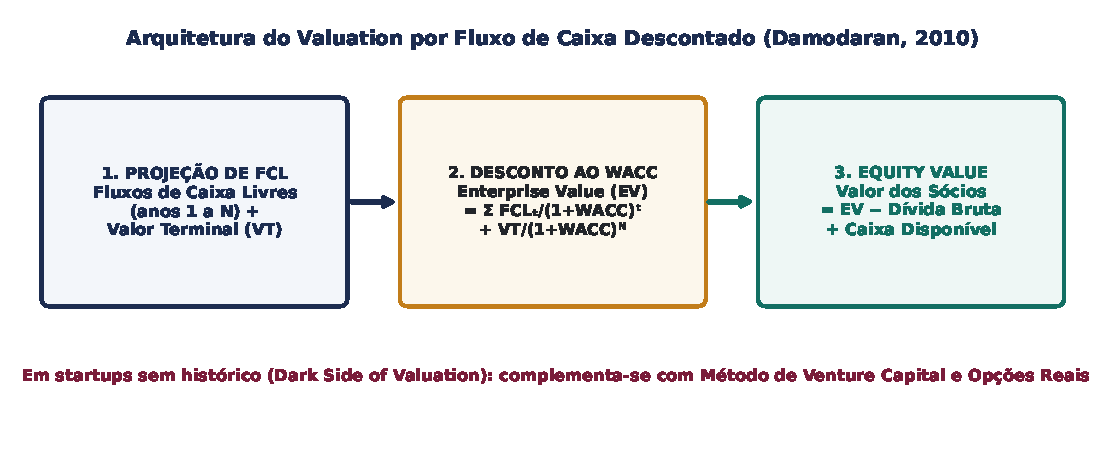
\includegraphics[width=0.94\textwidth]{figures/fig14_valuation_fcd_vc.pdf}
  \caption{Arquitetura de Valuation: Fluxo de Caixa Descontado (WACC, Gordon, EV e Equity) versus Método de Venture Capital.}
  \label{fig:14_valuation}
\end{figure}

\subsection{\textit{The Dark Side of Valuation}, Venture Capital e Opções Reais}

Quando tentamos aplicar o FCD tradicional a startups nascentes, de base tecnológica ou projetos de impacto em estágio pré-operacional, enfrentamos o que Damodaran (2010) denomina \textit{The Dark Side of Valuation}: ausência de histórico contábil, fluxos de caixa negativos nos primeiros anos, alta taxa de mortalidade e incerteza sobre o tamanho futuro do mercado. Nesses casos, dois instrumentos complementam ou substituem o FCD:

\begin{boxConceito}[Método de Venture Capital e Opções Reais]
\begin{enumerate}[leftmargin=1.4em, itemsep=3pt]
  \item \textbf{Método de Venture Capital (VC):} o fundo parte do futuro para o presente. Estima o \textbf{Valor de Saída ($EV_{\text{saída}}$)} em um horizonte $n$ (tipicamente $3$ a $7$ anos) aplicando um múltiplo de mercado (ex.: $EV/EBITDA$ ou $EV/\text{Receita}$) sobre a métrica projetada. Em seguida, desconta esse valor pela \textbf{TIR-alvo do fundo} ($r_{VC}$, alta para compensar o risco do portfólio):
  \[
    \text{Post-money} = \frac{\text{Valor de Saída}}{(1 + r_{VC})^n}, \qquad \text{Pre-money} = \text{Post-money} - \text{Aporte}, \qquad \%\text{Participação} = \frac{\text{Aporte}}{\text{Post-money}}
  \]
  \item \textbf{Opções Reais:} diferente do VPL estático (que assume decisão rígida ``agora ou nunca''), a teoria de Opções Reais incorpora o valor econômico da \textbf{flexibilidade gerencial}: o direito, mas não a obrigação, de \textbf{adiar} o investimento aguardando redução de incerteza, \textbf{expandir} a planta se a demanda superar o esperado, ou \textbf{abandonar} o projeto vendendo ativos caso o cenário seja adverso. Assim:
  \[
    VPL_{\text{expandido}} = VPL_{\text{estático}} + \text{Valor da Opção Real}
  \]
\end{enumerate}
\end{boxConceito}

\etapa{4}{Exemplos Resolvidos Passo a Passo}

\begin{boxExemplo}{14.1}{Cálculo do Custo Médio Ponderado de Capital (WACC)}
\passoEnunciado{Uma empresa de tecnologia limpa instalada em parque tecnológico regional financia suas operações com capital próprio e dívida de longo prazo junto a banco de fomento.}
\passoDados{Valor de mercado do Patrimônio Líquido ($E$) = \reais{6.000.000}; Dívida onerosa ($D$) = \reais{4.000.000}; Custo do capital próprio ($K_e$) = $16\%$ a.a.; Custo da dívida antes dos impostos ($K_d$) = $10\%$ a.a.; Alíquota efetiva de IR/CSLL ($T$) = $34\%$.}
\passoPedido{Calcular os pesos de capital ($E/(D+E)$ e $D/(D+E)$) e o $WACC$ anual da empresa.}
\passoMetodo{Cálculo da estrutura de capital total ($D+E$), aplicação do escudo fiscal na dívida $K_d(1-T)$ e média ponderada.}
\passoContas{%
\begin{align*}
  D + E &= 4.000.000 + 6.000.000 = \reais{10.000.000} \\
  \frac{E}{D + E} &= \frac{6.000.000}{10.000.000} = 0{,}60 \ (60\%), \qquad \frac{D}{D + E} = \frac{4.000.000}{10.000.000} = 0{,}40 \ (40\%) \\[4pt]
  K_d (1 - T) &= 10\% \times (1 - 0{,}34) = 10\% \times 0{,}66 = 6{,}60\% \\[4pt]
  WACC &= (0{,}60 \times 16\%) + (0{,}40 \times 6{,}60\%) \\
  &= 9{,}60\% + 2{,}64\% = 12{,}24\%\text{ a.a.}
\end{align*}
}
\passoResposta{O Custo Médio Ponderado de Capital ($WACC$) é de \textbf{12,24\% a.a.}}
\passoVerificacao{O $WACC$ ($12{,}24\%$) situa-se entre o custo líquido da dívida ($6{,}60\%$) e o custo do capital próprio ($16\%$), refletindo exatamente o peso de $60\%$ de sócios e $40\%$ de credores.}
\end{boxExemplo}

\begin{boxExemplo}{14.2}{Valuation Completo por FCD: Gordon, Enterprise Value e Equity Value}
\passoEnunciado{Um fundo de investimento avalia a aquisição de uma empresa de automação agrícola que possui projeção explícita de FCL para os próximos $3$ anos.}
\passoDados{$FCL_1 = \reais{500.000}$, $FCL_2 = \reais{600.000}$, $FCL_3 = \reais{720.000}$. $WACC = 12\%$ a.a.; taxa de crescimento perpétuo após o Ano $3$ ($g$) = $3\%$ a.a. A empresa possui Dívida Bruta de \reais{1.500.000}, Caixa de \reais{300.000} e $1.000.000$ de ações emitidas.}
\passoPedido{Calcular o Valor Presente dos FCLs explícitos, o Valor Terminal ($VT_3$), o $EV$, o $Equity\ Value$ e o valor justo por ação.}
\passoMetodo{Desconto individual de $FCL_1, FCL_2, FCL_3$ a $12\%$; aplicação da perpetuidade de Gordon em $t=3$; desconto de $VT_3$ por $(1{,}12)^3$; ajuste de dívida e caixa.}
\passoContas{%
\begin{align*}
  VP(FCL_{1..3}) &= \frac{500.000}{1{,}12} + \frac{600.000}{1{,}12^2} + \frac{720.000}{1{,}12^3} \\
  &= 446.428{,}57 + 478.316{,}33 + 512.481{,}78 = \reais{1.437.226{,}68} \\[6pt]
  VT_3 &= \frac{720.000 \times (1 + 0{,}03)}{0{,}12 - 0{,}03} = \frac{741.600}{0{,}09} = \reais{8.240.000{,}00} \\
  VP(VT_3) &= \frac{8.240.000}{1{,}12^3} = \frac{8.240.000}{1{,}404928} = \reais{5.865.069{,}24} \\[6pt]
  EV &= 1.437.226{,}68 + 5.865.069{,}24 = \reais{7.302.295{,}92} \\
  Equity &= 7.302.295{,}92 - 1.500.000 + 300.000 = \reais{6.102.295{,}92} \\
  \text{Preço justo por ação} &= \frac{6.102.295{,}92}{1.000.000} \approx \reais{6{,}10/\text{ação}}
\end{align*}
}
\passoResposta{$EV = \mathbf{\reais{7.302.295{,}92}}$; $Equity\ Value = \mathbf{\reais{6.102.295{,}92}}$; Valor por ação = \textbf{\reais{6,10}}.}
\passoVerificacao{Note que $VP(VT_3)$ representa $80{,}3\%$ do $EV$ total ($\frac{5{,}865}{7{,}302}$), fenômeno clássico em \textit{Valuation} que exige rigor na escolha de $g$ (nunca superior ao crescimento nominal de longo prazo da economia).}
\end{boxExemplo}

\begin{boxExemplo}{14.3}{Método de Venture Capital: Post-money, Pre-money e Participação}
\passoEnunciado{Uma healthtech universitária busca um aporte de \reais{2.000.000} junto a um fundo de Venture Capital para escalar sua plataforma de telemonitoramento no SUS regional.}
\passoDados{Aporte solicitado = \reais{2.000.000}; horizonte de saída do fundo ($n$) = $4$ anos; EBITDA projetado no Ano $4$ = \reais{2.500.000}; múltiplo setorial de saída ($EV/EBITDA$) = $8\times$; TIR-alvo exigida pelo fundo ($r_{VC}$) = $40\%$ a.a. (sem dívida ou caixa relevantes na saída).}
\passoPedido{Calcular o Valor de Saída, o \textit{Post-money Valuation}, o \textit{Pre-money Valuation} e o percentual de participação societária exigido pelo fundo.}
\passoMetodo{Cálculo de $\text{Saída} = EBITDA_4 \times 8$; desconto por $(1{,}40)^4$ para achar o \textit{Post-money}; subtração do aporte para o \textit{Pre-money}; divisão $\text{Aporte}/\text{Post-money}$.}
\passoContas{%
\begin{align*}
  \text{Valor de Saída (Ano 4)} &= 2.500.000 \times 8 = \reais{20.000.000{,}00} \\[4pt]
  \text{Post-money} &= \frac{20.000.000}{(1{,}40)^4} = \frac{20.000.000}{3{,}8416} = \reais{5.206.164{,}10} \\[4pt]
  \text{Pre-money} &= 5.206.164{,}10 - 2.000.000 = \reais{3.206.164{,}10} \\[4pt]
  \%\text{Participação do Fundo} &= \frac{2.000.000}{5.206.164{,}10} \times 100\% = 38{,}42\%
\end{align*}
}
\passoResposta{Saída = \textbf{\reais{20,00 mi}}; \textit{Post-money} = \textbf{\reais{5.206.164,10}}; \textit{Pre-money} = \textbf{\reais{3.206.164,10}}; Participação exigida = \textbf{38,42\%}.}
\passoVerificacao{Se os fundadores aceitarem ceder $38{,}42\%$ hoje, em $4$ anos essa fatia valerá $0{,}3842 \times 20.000.000 = \reais{7.684.000}$, entregando exatamente os $40\%$ ao ano compostos sobre os \reais{2,00 mi} investidos ($2{,}0 \times 3{,}8416 = 7{,}6832\text{ mi}$).}
\end{boxExemplo}

\begin{boxExemplo}{14.4}{Dark Side of Valuation: Múltiplo de Receita Recorrente (ARR) em Startup Inicial}
\passoEnunciado{Uma agtech SaaS (software como serviço para gestão de cooperativas) possui apenas $18$ meses de operação, margem EBITDA ainda negativa ($-\reais{300.000/\text{ano}}$) devido a gastos de P\&D, mas forte tração comercial.}
\passoDados{Receita Recorrente Anual ($ARR$) atual = \reais{1.200.000}; crescimento anual de $50\%$; empresas SaaS comparáveis no mercado brasileiro negociam a um múltiplo mediano $EV/ARR = 4{,}0\times$.}
\passoPedido{Explicar por que o FCD tradicional com base no lucro atual falha e estimar o $EV$ referencial pelo múltiplo de $ARR$.}
\passoMetodo{Aplicação de avaliação relativa por múltiplo de receita ($EV = ARR \times \text{Múltiplo}$), típica de startups em estágio de crescimento com margem negativa.}
\passoContas{%
\[
  EV_{\text{ARR}} = 1.200.000 \times 4{,}0 = \reais{4.800.000{,}00}
\]
}
\passoResposta{$EV$ referencial de \textbf{\reais{4.800.000,00}}.}
\passoVerificacao{Um múltiplo de $EBITDA$ seria impossível (geraria valor negativo). O múltiplo de $ARR$ contorna o \textit{Dark Side of Valuation} no curto prazo, desde que a startup apresente economia unitária saudável ($LTV > 3 \times CAC$) que garanta lucratividade futura.}
\end{boxExemplo}

\begin{boxExemplo}{14.5}{Opções Reais: Valor da Flexibilidade de Abandono em Biorrefinaria}
\passoEnunciado{Um projeto piloto de biorrefinaria de resíduos agroindustriais exige investimento inicial $I_0 = \reais{1.000.000}$. No Ano $1$, o mercado se define com igual probabilidade ($50\%$) entre um cenário favorável (Valor Presente dos fluxos futuros em $t=1$ igual a \reais{1.600.000}) e um cenário adverso (Valor Presente igual a \reais{600.000}). A $TMA$ é de $10\%$ a.a.}
\passoDados{$I_0 = \reais{1.000.000}$; $p_{\text{bom}} = 0{,}50$ ($V_1 = 1.600.000$); $p_{\text{ruim}} = 0{,}50$ ($V_1 = 600.000$); $TMA = 10\%$. Entretanto, o contrato permite \textbf{abandonar} o projeto no Ano $1$ e liquidar os equipamentos modulares por \reais{800.000}.}
\passoPedido{Calcular o $VPL_{\text{estático}}$ (sem opção de abandono), o $VPL_{\text{expandido}}$ (com opção de abandono) e o Valor da Opção Real ($VOR$).}
\passoMetodo{Cálculo do valor esperado em $t=1$ sem flexibilidade e com substituição do payoff adverso pelo valor de liquidação ($\max(600.000;\, 800.000) = 800.000$), descontado a $10\%$.}
\passoContas{%
\begin{align*}
  VPL_{\text{estático}} &= \frac{(0{,}50 \times 1.600.000) + (0{,}50 \times 600.000)}{1{,}10} - 1.000.000 \\
  &= \frac{800.000 + 300.000}{1{,}10} - 1.000.000 = \frac{1.100.000}{1{,}10} - 1.000.000 = \reais{0{,}00} \\[6pt]
  VPL_{\text{expandido}} &= \frac{(0{,}50 \times 1.600.000) + (0{,}50 \times \max(600.000;\, 800.000))}{1{,}10} - 1.000.000 \\
  &= \frac{800.000 + 400.000}{1{,}10} - 1.000.000 = \frac{1.200.000}{1{,}10} - 1.000.000 \\
  &= 1.090.909{,}09 - 1.000.000 = +\reais{90.909{,}09} \\[6pt]
  VOR &= VPL_{\text{expandido}} - VPL_{\text{estático}} = 90.909{,}09 - 0 = \reais{90.909{,}09}
\end{align*}
}
\passoResposta{$VPL_{\text{estático}} = \mathbf{\reais{0{,}00}}$; $VPL_{\text{expandido}} = \mathbf{+\reais{90.909{,}09}}$; Valor da Opção Real de Abandono = \textbf{\reais{90.909,09}}.}
\passoVerificacao{Pela análise estática ($VPL = 0$), o projeto seria indiferente e provavelmente descartado. Ao incorporar equipamentos modulares com mercado secundário (flexibilidade de abandono), o risco de perda extrema é limitado e o projeto passa a criar \reais{90.909,09} de valor líquido.}
\end{boxExemplo}

\etapa{5}{Armadilhas Conceituais e Erros Mais Comuns}

\begin{boxErro}[Erro 1: Assumir taxa de crescimento perpétuo $g \ge WACC$ na fórmula de Gordon]
Se $g \ge WACC$, o denominador $(WACC - g)$ torna-se zero ou negativo, produzindo valor infinito ou negativo absurdo. Além disso, nenhuma empresa pode crescer perpetuamente acima do PIB nominal da economia sem se tornar maior que o próprio mercado.
\end{boxErro}

\begin{boxErro}[Erro 2: Esquecer o benefício fiscal da dívida $(1 - T)$ no WACC]
Os juros pagos sobre empréstimos são dedutíveis da base de cálculo do IR/CSLL no lucro real. Usar $K_d$ bruto em vez de $K_d(1-T)$ superestima o WACC e subestima o $Enterprise\ Value$.
\end{boxErro}

\begin{boxErro}[Erro 3: Confundir Enterprise Value ($EV$) com Equity Value ($Equity$)]
Ao vender $100\%$ das quotas ou negociar uma rodada de investimento, o valor que pertence aos acionistas é o \textbf{Equity Value} ($EV - \text{Dívida Bruta} + \text{Caixa}$), não o $EV$. Ignorar a dívida na negociação faz o comprador assumir passivos sem ajuste de preço.
\end{boxErro}

\begin{boxErro}[Erro 4: Usar $FCL_n$ em vez de $FCL_{n+1}$ no numerador de Gordon]
Na perpetuidade de Gordon aplicada ao final do ano $n$, o numerador exige o fluxo do primeiro ano da perpetuidade: $FCL_{n+1} = FCL_n (1+g)$. Esquecer o fator $(1+g)$ subestima o Valor Terminal.
\end{boxErro}

\etapa{6}{Lista de Exercícios de Fixação (15 Questões)}

\begin{enumerate}[leftmargin=1.6em, itemsep=5pt]
  \item Diferencie \textbf{preço} de \textbf{valor intrínseco} segundo Damodaran (2010), explicando por que uma startup pode ser negociada a um preço acima ou abaixo de seu valor fundamental. \espacoResolucao[1.5cm]
  \item Calcule o custo do capital próprio ($K_e$) pelo modelo CAPM sabendo que a taxa livre de risco ($R_f$) é $10\%$ a.a., o beta ($\beta$) setorial é $1{,}2$ e o prêmio de risco de mercado ($R_m - R_f$) é $5\%$ a.a. \espacoResolucao[1.5cm]
  \item Uma empresa tem estrutura de capital composta por $70\%$ de capital próprio ($K_e = 15\%$ a.a.) e $30\%$ de dívida ($K_d = 10\%$ a.a.), com alíquota de IR/CSLL $T = 34\%$. Calcule o $WACC$. \espacoResolucao[1.6cm]
  \item Uma firma gera $FCL_n = \reais{400.000}$ no último ano do horizonte explícito, com crescimento perpétuo $g = 4\%$ a.a. e $WACC = 12\%$ a.a. Calcule o Valor Terminal ($VT_n$) pela perpetuidade de Gordon. \espacoResolucao[1.6cm]
  \item Sabendo que o \textit{Enterprise Value} ($EV$) de uma empresa é \reais{8.500.000}, sua Dívida Bruta é de \reais{2.200.000} e seu Caixa disponível é de \reais{700.000}, calcule o \textit{Equity Value}. \espacoResolucao[1.5cm]
  \item Calcule o $EV$ completo de uma startup madura com $FCL_1 = \reais{300.000}$, $FCL_2 = \reais{360.000}$, $WACC = 10\%$ a.a. e crescimento perpétuo $g = 2\%$ a.a. após o Ano $2$. \espacoResolucao[2.0cm]
  \item Pelo Método de Venture Capital, um fundo projeta que uma edtech valerá \reais{12.500.000} na saída no Ano $3$ e exige uma TIR-alvo de $50\%$ a.a. Se o fundo aportar \reais{1.000.000} hoje, calcule o \textit{Post-money}, o \textit{Pre-money} e a participação societária (\%) exigida. \espacoResolucao[1.9cm]
  \item Um empreendedor detém $100\%$ de sua startup. Na rodada Seed, vende $20\%$ da empresa para um investidor anjo. Dois anos depois, na Série A, um fundo entra adquirindo $25\%$ da empresa (diluição proporcional). Qual será a participação final do fundador após a Série A? \espacoResolucao[1.6cm]
  \item Um projeto possui $VPL_{\text{estático}} = -\reais{100.000}$ ($VP = \reais{900.000}$ e $I_0 = \reais{1.000.000}$). Entretanto, no Ano $1$, com probabilidade de $40\%$, a empresa pode exercer uma \textbf{opção real de expansão}: investir \reais{400.000} adicionais para gerar um valor presente adicional de \reais{950.000} em $t=1$. À $TMA = 10\%$ a.a., qual é o $VPL_{\text{expandido}}$? \espacoResolucao[1.9cm]
  \item Por que o modelo FCD apresenta limitações severas (\textit{The Dark Side of Valuation}) quando aplicado a startups pré-operacionais ou projetos de P\&D profundo? \espacoResolucao[1.5cm]
  \item Explique por que o Valor Terminal costuma responder por $60\%$ a $85\%$ do $EV$ total em empresas em crescimento e qual o risco de inflar a taxa $g$ na avaliação. \espacoResolucao[1.5cm]
  \item Em negócios de impacto territorial (como cooperativas tecnológicas ou bioeconomia), como o retorno socioambiental não precificado no FCL dialoga com o valor econômico estimado? \espacoResolucao[1.5cm]
  \item Qual é a diferença conceitual entre descontar o $FCL$ pelo $WACC$ (para achar o $EV$) e descontar o Valor de Saída pela TIR-alvo no Método de Venture Capital? \espacoResolucao[1.5cm]
  \item Cite e exemplifique os três tipos principais de Opções Reais em projetos tecnológicos: opção de adiar, opção de expandir e opção de abandonar. \espacoResolucao[1.5cm]
  \item Se uma empresa possui mais Caixa do que Dívida Bruta (Dívida Líquida negativa), o seu \textit{Equity Value} será maior ou menor que o seu \textit{Enterprise Value}? Justifique pela equação contábil. \espacoResolucao[1.5cm]
\end{enumerate}

\etapa{7}{Desafios Autorais e Aplicação Territorial (Preparação AV3)}

\begin{enumerate}[leftmargin=1.6em, itemsep=5pt]
  \item \textbf{Valuation do Projeto da AV3:} Estime o $EV$ e o $Equity\ Value$ do empreendimento do seu grupo utilizando o FCD em $3$ a $5$ anos com perpetuidade conservadora ($g \le 3\%$ a.a.), explicitando a composição do $WACC$. \espacoResolucao[2.0cm]
  \item \textbf{Simulação de Rodada de Investimento:} Suponha que seu grupo precise captar o CAPEX inicial via investidor-anjo ou fundo de impacto com TIR-alvo de $30\%$ a.a. em $4$ anos. Calcule qual percentual societário seria cedido pelo Método de Venture Capital e avalie se a diluição é aceitável para os fundadores. \espacoResolucao[1.9cm]
  \item \textbf{Flexibilidade Territorial:} Identifique uma Opção Real concreta no projeto da AV3 (ex.: implantar em módulos escaláveis conforme adesão da cooperativa ou manter opção de uso alternativo do galpão) e explique como ela reduz o risco de perda máxima. \espacoResolucao[1.6cm]
\end{enumerate}

\begin{boxDica}[Contraponto Crítico e Prática Territorial (AV2 e AV3)]
Ao apresentar um \textit{Valuation} para investidores ou bancos de fomento, evite ``planilhas mágicas'' em que o Valor Terminal justifica sozinho um negócio deficitário nos primeiros cinco anos. Mostre em quanto tempo o negócio atinge o equilíbrio operacional (Cap. 12), qual é o VPL dos fluxos explícitos (Cap. 13) e qual é o múltiplo implícito na saída (Cap. 14).
\end{boxDica}

\clearpage
\etapa{8}{Gabarito Integralmente Comentado (Exercícios 1 a 15 + Desafios 1 a 3)}

\begin{boxGabarito}[Resolução Passo a Passo — Exercícios de Fixação (1 a 15)]
\begin{enumerate}[leftmargin=1.5em, itemsep=4pt]
  \item \textbf{Preço vs. Valor:} Valor intrínseco reflete a geração futura de caixa descontada pelo risco; preço é o resultado da negociação de mercado em dado momento, podendo desviar-se do valor por escassez de liquidez, euforia ou assimetria de informação.
  \item \textbf{CAPM:} $K_e = 10\% + 1{,}2 \times 5\% = 10\% + 6\% = \mathbf{16{,}00\%\text{ a.a.}}$.
  \item \textbf{WACC:} $WACC = (0{,}70 \times 15\%) + (0{,}30 \times 10\% \times (1 - 0{,}34)) = 10{,}50\% + 1{,}98\% = \mathbf{12{,}48\%\text{ a.a.}}$.
  \item \textbf{Gordon:} $FCL_{n+1} = 400.000 \times 1{,}04 = \reais{416.000}$. $VT_n = 416.000 / (0{,}12 - 0{,}04) = 416.000 / 0{,}08 = \mathbf{\reais{5.200.000}}$.
  \item \textbf{EV para Equity:} $Equity = 8.500.000 - 2.200.000 + 700.000 = \mathbf{\reais{7.000.000}}$.
  \item \textbf{FCD completo:}
  $VT_2 = \frac{360.000 \times 1{,}02}{0{,}10 - 0{,}02} = \frac{367.200}{0{,}08} = \reais{4.590.000}$. \\
  $EV = \frac{300.000}{1{,}10} + \frac{360.000 + 4.590.000}{1{,}10^2} = 272.727{,}27 + \frac{4.950.000}{1{,}21} = 272.727{,}27 + 4.090.909{,}09 = \mathbf{\reais{4.363.636{,}36}}$.
  \item \textbf{Venture Capital:}
  $\text{Post-money} = \frac{12.500.000}{1{,}50^3} = \frac{12.500.000}{3{,}375} = \mathbf{\reais{3.703.703{,}70}}$. \\
  $\text{Pre-money} = 3.703.703{,}70 - 1.000.000 = \mathbf{\reais{2.703.703{,}70}}$. \\
  $\%\text{Participação} = \frac{1.000.000}{3.703.703{,}70} \times 100\% = \mathbf{27{,}00\%}$.
  \item \textbf{Diluição:} Após Seed, fundador mantém $80\%$. Na Série A, novos investidores ficam com $25\%$, restando $75\%$ para os acionistas anteriores: $0{,}80 \times 0{,}75 = \mathbf{60{,}00\%}$ para o fundador.
  \item \textbf{Opção de Expansão:} No Ano $1$, o ganho líquido da expansão é $950.000 - 400.000 = \reais{550.000}$ (positivo, logo a opção é exercida se o cenário ocorrer). $VP(\text{Opção}) = \frac{0{,}40 \times 550.000}{1{,}10} = \frac{220.000}{1{,}10} = \reais{200.000}$. Assim, $VPL_{\text{expandido}} = -100.000 + 200.000 = \mathbf{+\reais{100.000}}$.
  \item \textbf{Dark Side:} Startups jovens não têm histórico de receita estável, operam com margens negativas, dependem de rodadas futuras incertas e têm alta taxa de fracasso, tornando o $FCL$ de curto prazo negativo e o $VT$ extremamente sensível a premissas especulativas.
  \item \textbf{Peso do VT:} Em empresas em expansão, o caixa se concentra no longo prazo após a maturação do CAPEX. Inflar $g$ reduz $(WACC - g)$ no denominador, multiplicando artificialmente o $VT$ e distorcendo o $EV$.
  \item \textbf{Impacto territorial:} O $Valuation$ financeiro mede o valor capturável em moeda pelo empreendimento; externalidades positivas (emprego local, conservação de solo/água, segurança alimentar) devem ser reportadas paralelamente por métricas de impacto (Cap. 5) para atrair capital paciente ou subvenção.
  \item \textbf{WACC vs. TIR-alvo VC:} O $WACC$ reflete o custo ponderado de capital de uma empresa em operação contínua com risco estabilizado. A TIR-alvo de VC ($30\%$ a $60\%$) incorpora o risco de mortalidade e iliquidez de startups, servindo como taxa de desconto ajustada ao portfólio do fundo.
  \item \textbf{Tipos de Opções Reais:} \textit{Adiar}: esperar definição regulatória ou preço de commodity antes de construir; \textit{Expandir}: instalar planta modular com capacidade de dobrar linha de produção se a demanda validar; \textit{Abandonar}: vender ativos ou sublocar estrutura caso o mercado fracasse.
  \item \textbf{Caixa > Dívida:} Pela equação $Equity = EV - \text{Dívida Bruta} + \text{Caixa}$, se $\text{Caixa} > \text{Dívida Bruta}$, soma-se um valor líquido positivo ao $EV$, logo o \textbf{Equity Value será maior que o Enterprise Value}.
\end{enumerate}
\end{boxGabarito}

\begin{boxGabarito}[Diretrizes de Resposta — Desafios Autorais (1 a 3)]
\begin{enumerate}[leftmargin=1.5em, itemsep=3pt]
  \item \textbf{Desafio 1:} Deve apresentar $WACC$ coerente com a estrutura de financiamento do projeto (ex.: parcela subsidiada FNE/BNDES como $D$ e capital dos sócios como $E$), calcular $VT_n$ com $g < WACC$ e realizar a passagem $EV \to Equity$.
  \item \textbf{Desafio 2:} Deve projetar uma métrica de saída realista ($EBITDA_4 \times \text{múltiplo}$), descontar por $(1{,}30)^4 = 2{,}8561$ para obter o \textit{Post-money} e discutir o equilíbrio entre capital captado e governança dos fundadores.
  \item \textbf{Desafio 3:} Deve demonstrar como a modularização de investimentos reduz o comprometimento irreversível de capital no Ano $0$, convertendo risco de perda fixa em opção estratégica de baixo custo.
\end{enumerate}
\end{boxGabarito}

\begin{boxResumo}
\begin{itemize}[leftmargin=1.4em, itemsep=2pt]
  \item \textit{Valuation} estima o \textbf{valor intrínseco} pelos fundamentos, distinto do \textbf{preço} negociado.
  \item No \textbf{FCD} (Damodaran, 2010), desconta-se o $FCL$ e o Valor Terminal de Gordon ($VT_n = \frac{FCL_{n+1}}{WACC - g}$) pelo $WACC$ para obter o $EV$, ajustando-se Dívida e Caixa para chegar ao $Equity\ Value$.
  \item Em startups sem histórico (\textit{Dark Side}), o \textbf{Método de Venture Capital} parte do valor de saída descontado pela TIR-alvo do fundo para definir \textit{Post-money}, \textit{Pre-money} e participação.
  \item \textbf{Opções Reais} quantificam o valor da flexibilidade gerencial de adiar, expandir ou abandonar projetos.
\end{itemize}
\end{boxResumo}

\begin{boxTeste}
\begin{enumerate}[leftmargin=1.5em, itemsep=4pt]
  \item Calcule o $WACC$ de uma empresa com $80\%$ de capital próprio ($K_e = 15\%$), $20\%$ de dívida ($K_d = 10\%$) e alíquota $T = 30\%$.
  \item Se $EV = \reais{5.000.000}$, Dívida Bruta = \reais{1.200.000} e Caixa = \reais{400.000}, qual é o \textit{Equity Value}?
  \item (\V/\F) Na fórmula de Gordon, a taxa de crescimento perpétuo $g$ deve ser estritamente menor que o $WACC$.
  \item (\V/\F) Na análise de Opções Reais, a flexibilidade gerencial de abandonar um projeto deficitário reduz seu valor em relação ao $VPL$ estático.
\end{enumerate}
\vspace{4pt}
\noindent\textbf{Gabarito do Checkpoint:} \textbf{1.} $WACC = 0{,}80(15\%) + 0{,}20(10\%)(1 - 0{,}30) = 12{,}00\% + 1{,}40\% = \mathbf{13{,}40\%\text{ a.a.}}$. \quad \textbf{2.} $Equity = 5.000.000 - 1.200.000 + 400.000 = \mathbf{\reais{4.200.000}}$. \quad \textbf{3.} \V. \quad \textbf{4.} \F\ (aumenta ou preserva valor ao limitar perdas nos cenários adversos).
\end{boxTeste}
